% TODO:
% - explain constraint encoding (Heule, sequential)
% - correct results
% - add auxiliary variables
\section{SAT Model}
\subsection{Decision variables}
Let $sts$ be a schedule analogous to $rb$ satisfying to the STS problem:
% The satisfiability task is formalized by the following categories of propositions:

\subsubsection{Satisfiability}
% \paragraph{\text{matches\_schedule}}
\begin{itemize}
    \item \textbf{matches\_schedule}\\
        For each period $p \in P$ and week $w \in W$:
        $$
        matches\_schedule_{p, w, m} = true
        $$
        if, and only if, the match $rb_{m, w}$ takes place in period $p$ of week $w$
    \item \textbf{matches\_to\_periods}\\
        For each period $p \in P$, $t_1 \in T$ and $t_2 \in T/\{t_1\}$:
        $$
        matches\_to\_periods_{t_1, t_2, p} = true
        $$
        if, and only if, $t_1$ plays against $t_2$ in period $p$
\end{itemize}
\subsubsection{Optimization}
\begin{itemize}
    \item \textbf{flip\_slot}\\
        For each period $p \in P$ and week $w \in W$:
        $$
        flip\_slot_{p, w} = true
        $$
        if, and only if, team $sts_{p, w, 1} = t_1$ plays away
    \item \textbf{matches\_to\_slots}\\
        For each period $p \in P$, $t_1 \in T$ and $t_2 \in T/\{t_1\}$:
        $$
        matches\_to\_slots_{t_1, t_2} = true
        $$
        if, and only if, $t_1$ plays away and $t_2$ plays at home
\end{itemize}

\subsection{Objective function}
Similarly to the other approaches, the objective is to minimize the absolute difference between the number of games played at home and away for each team.
Let $A_t$ be the number of times the team $t \in T$ plays away, the objective function translates into the following:
$$
k^* = \underset{k \in \mathbb{N}}{\text{argmax}} \left( \forall t \in T, A_t \geq k \right)
$$
The chosen model allows to solve the optimization task using the $sts$ schedule computed in the satisfiability process. The optimization consists of a binary search of $k^*$ in the interval $[1, \lfloor\frac{N-1}{2}\rfloor]$. Since SAT doesn't directly support optimization, a new set of optimizing constraints is introduced for every instance of $k$ .

The result is encoded in $flip\_slot_{p, w}$, which cannot express the constraints alone, due to structural limitations of the encoding.
Instead \\$matches\_to\_slots_{t_1, t_2}$ is used: given a week $w$ and a period $p$, the team $sts_{p, w, 1} = t_1$ plays away if, and only if, the team $t_2 = sts_{p, w, 2}$ plays at home. Therefore, by definition:
$$
    \forall p \in P, w \in W.(flip\_slot_{p, w} \leftrightarrow matches\_to\_slots_{sts_{p, w, 1}, sts_{p, w, 2}})
$$
Finally the optimization process is implemented by ensuring that for an instance $k \in [1, \lfloor\frac{N-1}{2}\rfloor]$:
$$
    \forall p \in P, t_1 \in T.(AtLeastK(matches\_to\_slots_{t_1, t_2} | t_2 \in T/\{t_1\}))
$$

\subsection{Constraints}
\subsubsection{Each match is assigned to a unique period each week}
In a Round-Robin tournament $rb$, each team plays exactly once a week. 
Therefore the only problem is to ensure that for each week $w$, every match $rb_{m, w} = (t_i, t_j)$ is assigned to exactly one period $p$.

We enforce that every match is scheduled once:
$$
    \forall p \in P, w \in W.(ExactlyOne(matches\_schedule_{p, w, m} | m \in P))
$$
Finally no two matches are scheduled in the same period. 

We ensure that each match is scheduled to a unique period $p$ in the week $w$.
$$
    \forall m \in P, w \in W. ExactlyOne(matches\_schedule_{p, w, m} | p \in P)
$$
\subsubsection{Every team plays at most twice in the same period}
The constraint cannot be expressed using directly $matches\_schedule_{p, w, m}$, due to structural limitations of the encoding. 
Instead, we introduce the literal $matches\_to\_periods_{t_1, t_2, p}$: given a week $w$, the match $rb_{m,w}$ is scheduled in period $p$ if, and only if, the match $(rb_{m, w, 1}, rb_{m, w, 2}) = (t_1, t_2)$ takes place in period $p$. Therefore, by definition: 
$$
    \forall p \in P, w \in W, m \in P.(matches\_schedule_{p, w, m} \leftrightarrow matches\_to\_periods_{rb_{m, w, 1}, rb_{m, w, 2}, p})
$$
Computationally this constraint soundly binds $matches\_schedule$ to \\$matches\_to\_periods$, which allow to express the main constraint:
$$
    \forall p \in P, t_1 \in T. AtMost2(matches\_to\_periods_{t_1, t_2, p} | t_2 \in T/\{t_1\})
$$
\subsection{Validation}
% See Section 2.4. The model \textbf{must} be implemented using at least Z3. Bonus points will be considered if a solver-independent language (e.g., Dimacs) is employed so as to play with different SAT solvers on the same model.
\subsubsection{Experimental design}
The model was written in Python by making use of the Z3 and the CVC5 library, which offers CaDiCaL and MiniSat as the underlying SAT solvers. The time elapsed to find an optimal solution, within the 300 second time limit, was measured and results presented in Fig.\ref{fig:SAT-result} . 
\subsubsection{Experimental results}
All solvers either find the optimal solution or no solution at all. Overall Z3 had the fastest and was able to solve the problems with higher $N$, reaching $N=20$. On the other hand CaDiCaL was the worst, failing at $N=12$, while MiniSat stopped at $N=14$

\begin{table}[H]
\centering
\small
{%
\begin{tabular}{|c|c|c|c|}
\toprule
\textbf{n} & \textbf{Z3} &\textbf{CaDiCaL} & \textbf{MiniSat} \\
\midrule
6  & 0   & 0   & 0   \\
8  & 0   & 0   & 0   \\
10 & 0   & 0   & 0   \\
12 & 0   & N/A & N/A \\
14 & 0   & N/A & N/A \\
16 & 1   & N/A & N/A \\
18 & 16  & N/A & N/A \\
20 & 221 & N/A & N/A \\
22 & N/A & N/A & N/A \\
\bottomrule
\end{tabular}
}
\caption{SAT optimization solver results}
\label{table:mip-results}
\end{table}

\begin{figure}[H]
    \centering
    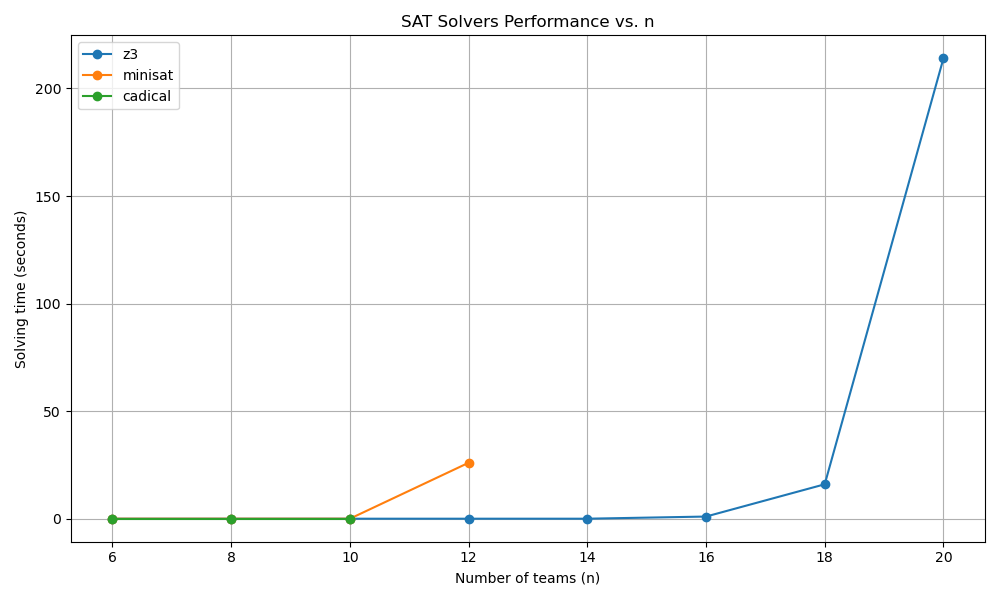
\includegraphics[width=0.8\linewidth]{img/SAT-result.png}
    \caption{SAT optimization}
    \label{fig:SAT-result}
\end{figure}
